\documentclass[12pt]{article}

\usepackage[utf8]{inputenc}
\usepackage{geometry}
\usepackage{graphicx}
\usepackage{hyperref}
\usepackage{listings}
\usepackage{wrapfig}
\usepackage{adjustbox}

\geometry{a4paper, margin=1in}

\title{Project Report: Cloud-Based File Storage System}
\author{Tanja Derin}
\date{\today}

\begin{document}

\maketitle

\tableofcontents


\section{Introduction}
\label{sec:introduction}
This project introduces a cloud-based file storage system that enables users to seamlessly upload, download, and delete files while ensuring the privacy of individual storage spaces. For efficiency and other purposes that will be discussed, Nextcloud has been selected for the deployment using Docker containers. MariaDB was used along with Docker and Nextcloud to provide reliable SQL database service. To ensure the service can handle real-world usage, Locust was employed to stress test the system, giving valuable insights into how Nextcloud performs under user traffic.

\subsection{Docker and Nextcloud}
\label{sec:Docker and Nextcloud}
Docker has been the main component of the deployment for this file storage system, offering a containerized framework for the operation of Nextcloud within isolated environments. The containers act as independent servers, each with the requisite elements for the autonomous operation of Nextcloud. Such design enhances deployment efficiency, facilitates updates, and simplifies scaling processes.

Central to the file storage solution is Nextcloud, which takes advantage of Docker’s offerings to deliver a suite of features, such as data encryption, file versioning, and collaborative tools that enhance user experience and system robustness. This Docker micro-service image is developed and maintained by the Nextcloud community, offering a variety of deployment options to suit different system setups. 

\begin{wrapfigure}{r}{0.40\textwidth}
  \centering
  
\includegraphics[width=0.45\textwidth]{Nextcloud_withDocker.png}
  \caption{Nextcloud and Docker}
  \label{fig:yourlabel}
\end{wrapfigure}


\section{System Architecture and Deployment}
\label{sec:deployment}
The deployment process begins with spinning up Docker containers, created from images that lay the foundation for our services. These images encapsulate the necessary software stacks, ensuring consistency across development.

The main component of the this system is the Nextcloud image, which bundles the file storage application with all its dependencies into a deployable unit, providing users with many features for managing and sharing files. Simultaneously, we employ a MariaDB image, chosen for its proven track record of reliability and scalability as a database service. This database acts as the persistent storage, crucial for maintaining user data and state across sessions.

Complementing these services, we introduce a container for Locust, an open-source load testing tool. This container is leveraging a custom Python script designed to mimic user behavior and interactions with Nextcloud. To run it we link to the necessary Python script, ensuring it targets the Nextcloud instance.

\subsection{Docker Compose}

The main role of the .yml file is orchestrating the Docker containers, it defines how the Nextcloud, MariaDB, and Locust containers should interact with one another. It specifies the configurations needed for each service, putting together environmental variables, volume mappings, and network settings to ensure that each container can fulfill its role effectively within the larger ecosystem.

\begin{wrapfigure}{l}{0.35\textwidth}
  \centering
  
\includegraphics[width=0.25\textwidth]{Docker-Compose-Logo.jpg}
  \caption{Docker compose}
  \label{fig:yourlabel}
\end{wrapfigure}


The docker-compose file allows to define the relationships between containers — for example, linking Nextcloud to MariaDB to ensure seamless data persistence and connectivity. Meanwhile, the Locust container is configured to communicate with Nextcloud, simulating user actions that test the system’s resilience and performance. The specification in this file are the following.
\begin{itemize}
    \item Networks, We specify custom networks to ensure that containers can communicate internally as if they were on a private subnet, isolating our services from external networks, which adds a layer of security and control. 
    \item Volumes, the volumes are defined to persist data, such as Nextcloud's files and MariaDB's database records, ensuring that the data remains intact across container restarts and updates.
    \item Dependencies, the configuration also establishes service dependencies, ensuring that services like Nextcloud wait for the MariaDB service to be fully up and running before they start.
\end{itemize}


%\subsubsection{Services}
%Each service, represented by a container, is configured with specific parameters. For Nextcloud, we ensure it connects to the appropriate database by setting environment variables that point to the MariaDB service.
%MariaDB is set up with its own environment variables, such as root and database user passwords, which are critical for securing access.


\subsection{Deployment}

To set up everything the 
\verb|docker-compose up| command is needed, which reads the script, pulls the required images, and creates the containers as defined. By running this single command, the entire environment is spun up, making it very straightforward to deploy a multi-container application. This process is one of the advantages of using Docker and docker-compose, allowing developers to deploy a fully-fledged cloud service with minimal fuss.

After setting up and starting the services with docker-compose up, there is one additional step required for Nextcloud configuration. To ensure Nextcloud recognizes and trusts the domain from which it is accessed to the simulated user generated by Locust. We execute an additional command:

%\begin{adjustbox}{max width=\textwidth}
\begin{verbatim}
docker exec --user www-data nextcloud php occ config:system:set
trusted_domains 1 --value=nextcloud
\end{verbatim}
%\end{adjustbox}

% Since Locust simulates user traffic, Nextcloud needs to recognize and accept requests from the domain where the Locust tests are originating. If the domain isn't listed as a trusted domain in Nextcloud's configuration, it could block the simulated traffic from Locust, rendering the tests ineffective.

Nextcloud becomes accessible at \url{http://localhost:8080}. This URL points the browser to the port 8080 on your the local machine, where Docker has mapped the internal port used by the Nextcloud container to be accessible from the host system.This makes it easy to interact with Nextcloud instance as if it were running directly on your machine, providing a direct way to manage files, users, and settings on its web interface.

The Locust testing framework becomes accessible at \url{http://localhost:8081}. Similar to how Nextcloud is set up, the Locust service is configured on a specific port inside its container, which Docker maps to 8081 on the host machine.

\section{Manage User, Files and Security}
\label{sec: Manage User and files}

Nextcloud's web interface stands out for its user-friendliness, allowing for straightforward user and file management tasks such as creating user accounts, assigning roles, and setting permissions, as well as uploading, downloading, and organizing files. This accessibility ensures that administrators can efficiently manage the cloud environment, while users enjoy a seamless experience in handling their data. 

Security is very important in a cloud-based file storage system, with a focus on ensuring both the secure storage and transmission of files, alongside robust user authentication measures to prevent unauthorized access.

User authentication security can be strengthened by the administrator through the enforcement of strong password policies and the implementation of two-factor authentication (2FA). These measures significantly reduce the risk of unauthorized access by adding an additional layer of security beyond just the password.


\begin{wrapfigure}{l}{0.38\textwidth}
  \centering
  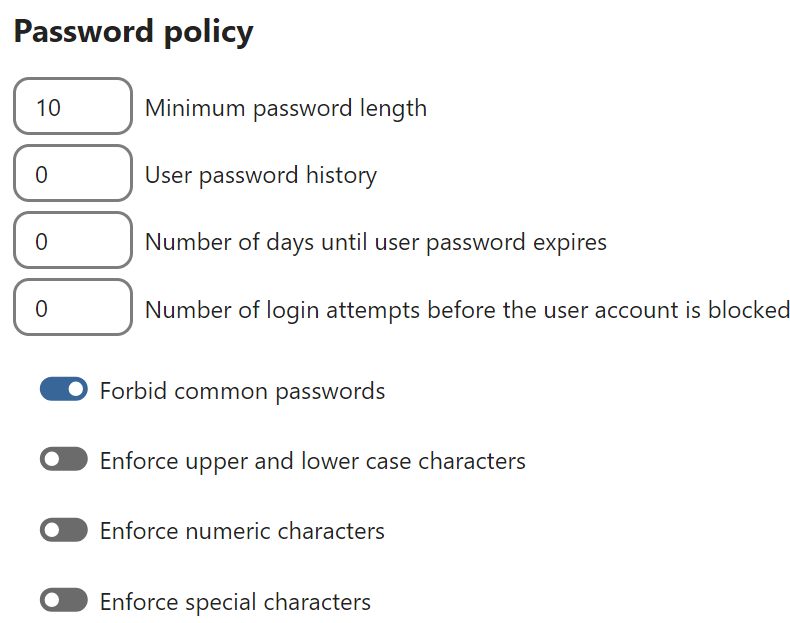
\includegraphics[width=0.28\textwidth]{Posnetek zaslona 2024-03-21 091850.png}
  \caption{Basic password policies}
  \label{fig:yourlabel}
\end{wrapfigure}


To secure file storage and transmission, one can utilize Nextcloud's encryption capabilities by implementing TLS (Transport Layer Security) protocols to encrypt data in transit, ensuring that file transfers between clients and the server are secure. This security measure is further strengthened by operating the system exclusively over HTTPS, leveraging the security benefits of SSL certificates to encrypt all communications. 

For data at rest, enabling server-side encryption (SSE) ensures that stored data is protected against external breaches. We can enable this with the command
\begin{verbatim}
    docker exec --user www-data $CONTAINER_ID php occ encryption:enable
\end{verbatim}
Following by the command,
\begin{verbatim}
    docker exec --user www-data $CONTAINER_ID php occ encryption:encrypt-all
\end{verbatim}
which ensures that all stored data, not just new data post-encryption activation, is secured against potential threats.

\begin{wrapfigure}{r}{0.45\textwidth}
  \centering
  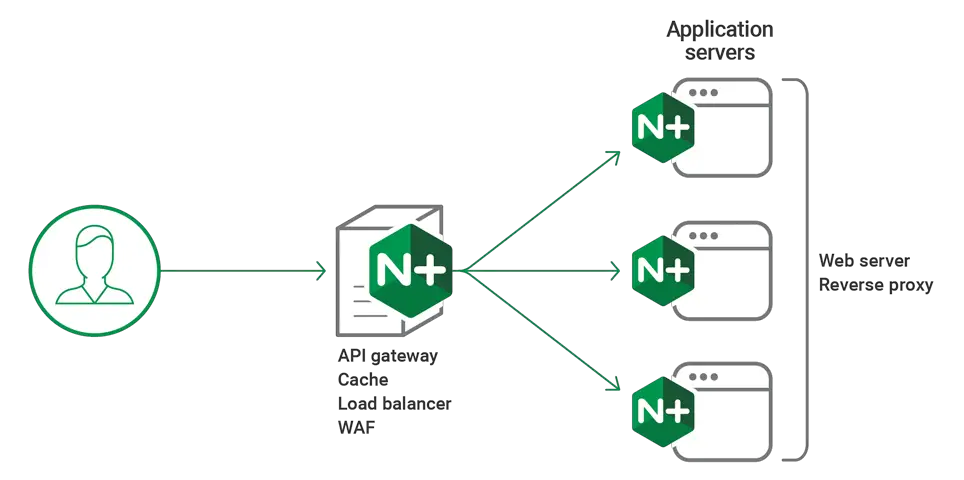
\includegraphics[width=0.45\textwidth]{Nginx_sec.png}
  \caption{Nginx}
  \label{fig:yourlabel}
\end{wrapfigure}

Additionally, using a reverse proxy like nginx boosts security by hiding the details of our backend servers from users. It also helps distribute traffic evenly, which improves system performance. In cloud-based architectures or when using external hosting services, a reverse proxy becomes an integral component of the infrastructure, managing the flow of information between the internet and the server hosting the application or website.

%\begin{wrapfigure}{r}{0.4\textwidth}
  %\centering
  %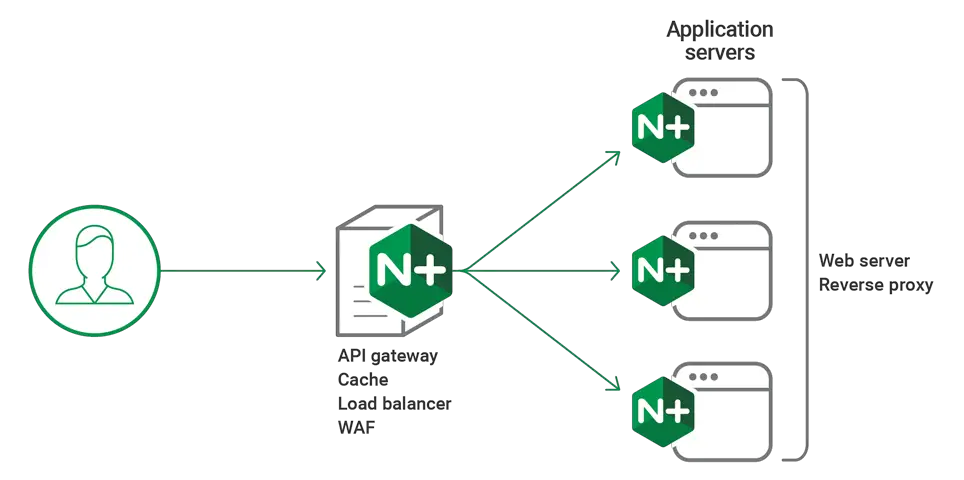
\includegraphics[width=0.4\textwidth]{Nginx_sec.png}
  %\caption{Nginx}
  %\label{fig:yourlabel}
%\end{wrapfigure}

%Additionally, the use of a reverse proxy, such as nginx, will not only enhance security by abstracting the backend server details from external users but also improve load balancing. By connecting our Docker instances to an established domain and managing SSL security policies through the reverse proxy, we ensure a secure, scalable, and efficient user-server communication framework.


\section{Efficiency and Scalability}
\label{sec:scalability}
\subsection{Efficiency}
In the the \verb|docker-compose.yml| the resource limitations are specified, such as CPU and memory allocations for the MariaDB (1 CPU and 500 MB), Nextcloud (2 CPU and 2000 MB) , and Locust (1 CPU and 1500 MB) containers. This are imposed due to the capabilities and constraints of the host computer. These limitations are ensuring that the system is efficient, resilient, and is also ensuring
\begin{itemize}
    \item Load balance, no single container can consume an excessive amount of the host's resources
    \item Stability and host protection, the constraints help in avoiding system overloads that could lead to crashes or degraded performance, so the containers collectively do not exhaust the host’s resources
    \item Development and Testing, for developers and testers, working within these defined limits provides a realistic understanding of how the system behaves under constrained conditions. 
\end{itemize}

Theoretically discussing the transition from personal computing resources to a more robust and shared infrastructure, to ensure efficiency while managing costs effectively, someone might opt for a hybrid cloud approach, combining on-premises hardware with cloud storage solutions. For data that is less sensitive or less frequently accessed, it utilizes cloud storage services provided by third parties like AWS S3, Azure Blob Storage, or Google Cloud Storage.

Additionally, by monitoring usage patterns and automatically adjusting resources scaling down during off-peak times and scaling up when demand increases small companies can ensure they pay only for the resources they need. 

\subsection{Scalability}

Exploring Nextcloud as a cloud-based file management solution underscores its adaptability across various organizational scales. Initially aimed at small to medium-sized enterprisesdue to its cost-free model, Nextcloud Server offers an invaluable resource for those looking to establish a solid digital infrastructure without incurring significant expenses. For larger entities requiring enhanced support and scalability options Nextcloud Enterprise as a suitable upgrade. This variant caters to a broad spectrum of organizational demands with its tiered service offerings.

To address potential server limitations as demands grow, overcoming the physical limitations of servers by implementing solutions that enhance the scalability of the server infrastructure itself. This includes
\begin{itemize}
    \item Vertical Scaling, increasing the capacity of existing servers by adding more resources (CPU, RAM, storage) to handle higher loads. This option may have limitations based on the maximum capacity of the hardware.
    \item Horizontal Scaling, Adding more server instances to distribute the load across multiple machines, thereby improving performance and reliability. This is often achieved through techniques like load balancing and clustering.
    \item Virtualization and Containerization: Using virtual machines (VMs) or containers to maximize the utilization of existing hardware and simplify the deployment and management of applications across multiple servers.
\end{itemize}

Adapting these insights into our project's framework it is important to choose a strategy that aligns with each entity's specific circumstances. Organizations with pre-existing infrastructure might find an on-premises deployment of Nextcloud or Nextcloud Enterprise, supplemented by cloud services during demand surges. Organizations just beginning to navigate their digital transformation might find the adaptability and cost efficiency of cloud platforms such as AWS particularly advantageous. AWS offers a range of services that provide virtual servers, storage, and networking capabilities, allowing organizations to build and scale their IT. This approach not only offers scalability and financial savvy but also guarantees that Nextcloud's deployment is attuned to the shifting demands of business operations. 

%opcije 
%-kupis serverje
%-rentas serverje
%-rentas memory

\section{Testing Infrastructure}
\label{sec:testing_infrastructure}

A Locust test is essentially just a Python program making requests to the system you want to test. This makes it very flexible and particularly good at implementing complex user flows. Methods decorated with @task are the locust file. For every running user, Locust creates a greenlet (micro-thread), that will call those methods.

The script creates user accounts and performs a series of tasks that mimic typical user interactions with the file storage system. These interactions include

\begin{itemize}
    \item User Creation, the script generates a unique username and password for a new user, then registers this user in the Nextcloud system, which tests the system's ability to handle new user registrations smoothly.
    
    \item Fetching file listings (\verb|get_files|), tests the system's response time and efficiency in listing user files, a common operation for users navigating their storage.
    
    \item Downloading a file (\verb|download_file|), simulates the downloading of a specific file 
    
    \item Uploading files of various sizes (\verb|upload_kb|,\verb| upload_mb|, \verb|upload_gb|), evaluate the system's capability to handle file uploads, from small files (1KB) to large ones (1GB)
    
\end{itemize}

The tasks are weighted to occur with different frequencies, reflecting their varying real-world usage patterns.


The testing was conducted via a Windows Subsystem for Linux (WSL) environment, on an ASUS ZenBook 14 equipped with 16 GB RAM, a 1TB storage capacity, and an i7 processor. It was observed that DockerWSL's resource consumption, particularly RAM usage reaching approximately $85\%$, potentially impacted the performance outcomes. This high memory utilization within the WSL context underscores the need for cautious interpretation of our test results, as the constrained resources not fully reflect the system's capabilities.

\begin{wrapfigure}{r}{0.57\textwidth}
  \centering
  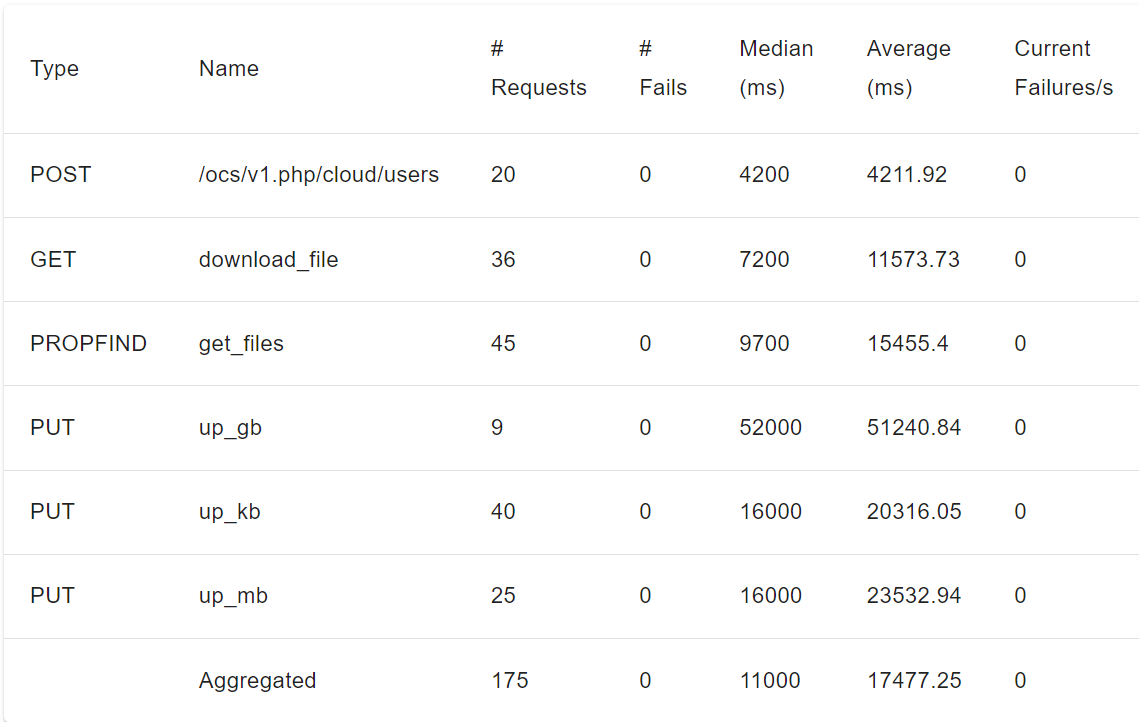
\includegraphics[width=0.57\textwidth]{Test_stat.png}
  \caption{Test statistics}
  \label{fig:yourlabel}
\end{wrapfigure}



For the test 20 users were simulated, with new users joining at the rate of one per second. The testing statistics provide a detailed view of the system's performance, user creation maintained zero failures, with median and average response times staying around 4200 ms, indicating a reliable user creation process. File download and retrieval operations (GET and PROPFIND requests) also showed zero failures but with higher response times, suggesting increased complexity or system load during these operations. Uploading files of varying sizes demonstrated the system's capacity to handle large files without failure, although the response time for a 1 GB file upload significantly spiked. 

\begin{figure}[ht]
\centering
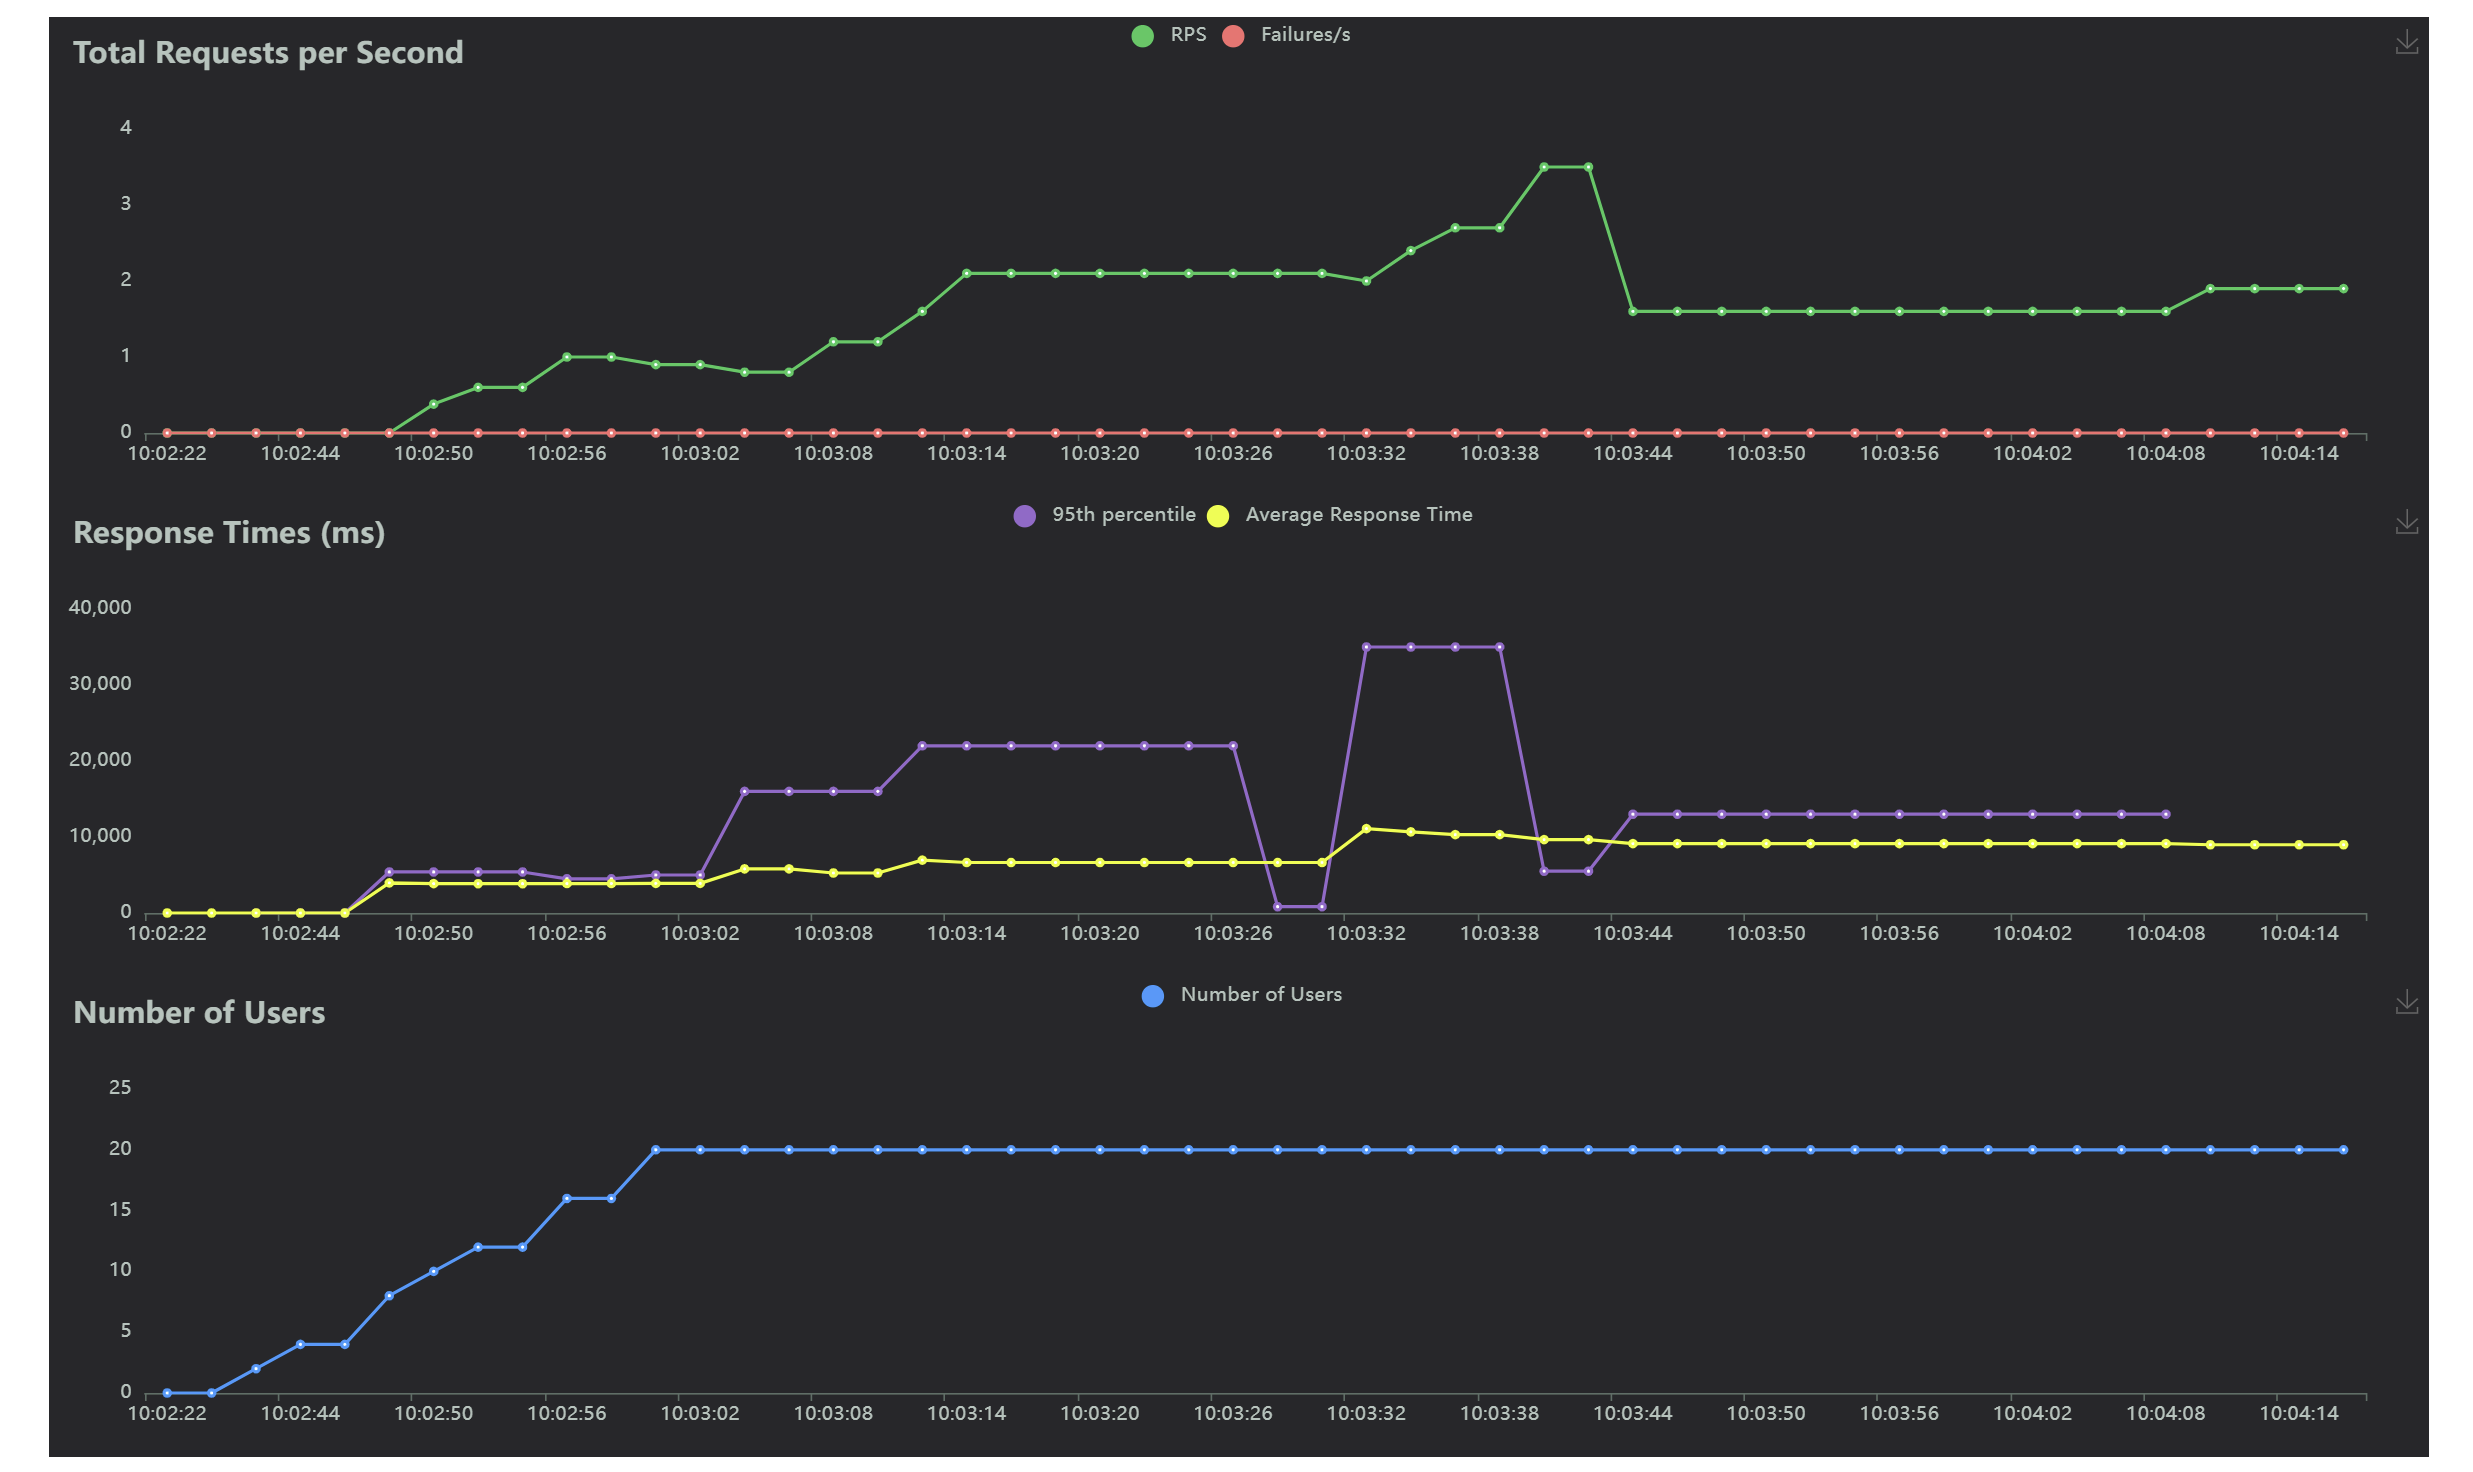
\includegraphics[width=\linewidth]{Test_20_1s.png}
\caption{Performance test results with 20 users at 1 user/second creation rate.}
\label{fig:testresults}
\end{figure}

The test results show a steady increase in total requests per second (RPS) with a delay respect to the creation of the users. Indicating that the system is taking some time to crate new users before handling the first requests, but its handling the growing number of users well, without significant failures. The response times is stable throughout the test, while the 95th percentile response time has occasional spikes, which may indicate specific operations like uploading large files. 

\begin{wrapfigure}{l}{0.4\textwidth}
  \centering
  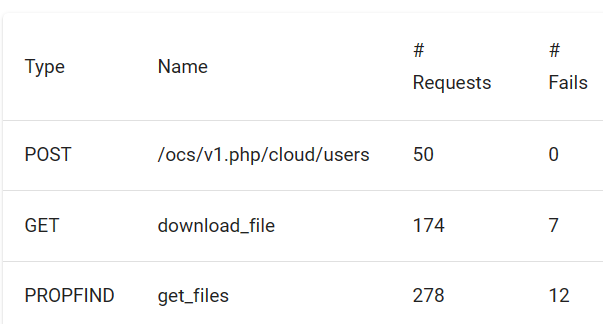
\includegraphics[width=0.38\textwidth]{Test2_stat.png}
  
  \label{fig:yourlabel}
\end{wrapfigure}
Another test was conducted with 50 users, created at a rate of 5 users per second and  sustained over a longer period. The outcomes were promising, with the system showing robust performance for the most part. Eventually, some requests failed after some time, indicating areas where further optimization may be needed.This test, along with additional ones are stored in a separate directory on the repository. 




\section{Conclusion}
\label{sec:conclusion}
The combination of Docker and Nextcloud yields a comprehensive solution, with Docker managing the operational environment and Nextcloud providing the functionality for users. The deployment strategy's adaptability allows both on-premises resources and cloud services, facilitating a flexible and economical file storage solution. This duality offers a solid foundation for small firms and individual users alike, providing a tailored experience that scales with organizational growth and technological evolution.

In the end, through monitoring, testing, and strategic upgrades, we can sustain a secure, scalable, and efficient service that responds to the emerging needs of our users.
\end{document}
